\chapter{Physics of lepton colliders}
\label{Lepton Physics}
\begin{chapterabstract}

\end{chapterabstract}
%\newline

\section{The Standard Model}
\label{StandardModel}
\section{Production modes}
\label{Production modes}
\section{Backgrounds}
\label{Backgrounds}
\subsection{High cross-section backgrounds from beam-beam interactions}
\label{BeamBeam}
\subsubsection{Pair background}
\label{BeamBeam:pairs}

\begin{figure}
\begin{subfigure}[b]{0.33\textwidth}
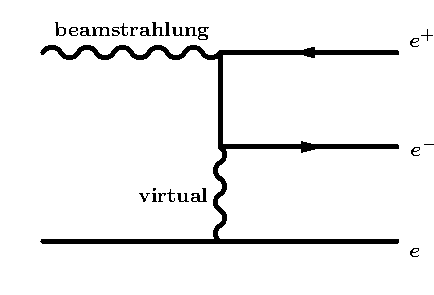
\includegraphics[width=\textwidth]{Figures/Bethe-Heitler.pdf}
\caption{Bethe-Heitler}
\end{subfigure}
\begin{subfigure}[b]{0.33\textwidth}
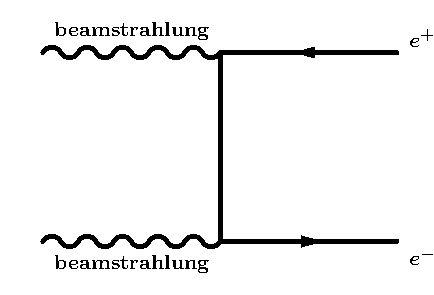
\includegraphics[width=\textwidth]{Figures/Breit-Wheeler.pdf}
\caption{Breit-Wheeler}
\end{subfigure}
\begin{subfigure}[b]{0.33\textwidth}
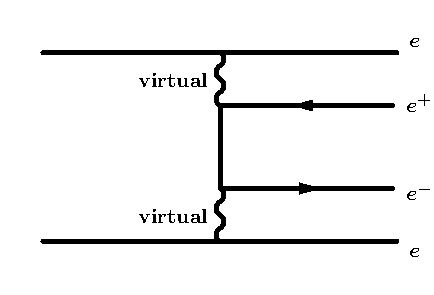
\includegraphics[width=\textwidth]{Figures/Landau-Lifshitz.pdf}
\caption{Landau-Lifschitz}
\end{subfigure}
\caption[LO Feynman diagrams of the production of the background pairs.]{The LO Feynman diagrams of the production processes of the background pairs: Bethe-Heitler, Breit-Wheeler and Landau-Lifschitz.}
\label{fig:Feynman:pair_production}
\end{figure}

\subsubsection{Bhabha scattering and $\gamma\gamma\rightarrow$hadrons}
\label{BeamBeam:bhabha_gammagamma}

\begin{figure}
\centering
\begin{subfigure}[b]{0.35\textwidth}
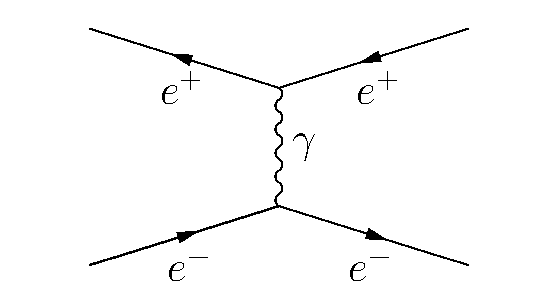
\includegraphics[width=\textwidth]{Figures/bhabha_scattering.pdf}
\caption{Bhabha scattering}
\end{subfigure}
\vspace*{0.2cm}
\begin{subfigure}[b]{0.35\textwidth}
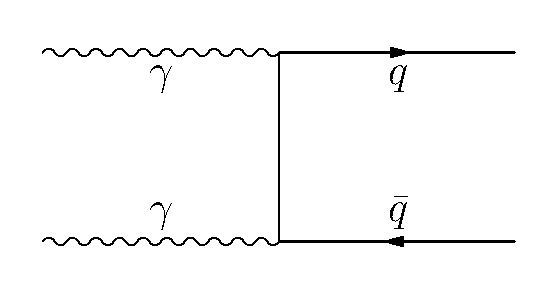
\includegraphics[width=\textwidth]{Figures/gammagamma_hadrons.pdf}
\caption{$\gamma\gamma\rightarrow$hadrons}
\end{subfigure}
\caption[LO Feynman diagrams of bhabha scattering and the $\gamma\gamma\rightarrow$hadrons process.]{The LO Feynman diagrams of the bhabha scattering and the $\gamma\gamma\rightarrow$hadrons process.}
\label{fig:Feynman:bhabha_gammagamma}
\end{figure}

\subsection{Machine backgrounds}
\label{MachineBackgrounds}